% https://userswww.pd.infn.it/~moretto/fontana/project/software/2018/03/16/compton-edge.html
\documentclass{article}
\usepackage[utf8]{inputenc}
\usepackage{blindtext}
\usepackage{graphicx}
\usepackage{amsmath}
\usepackage{csvsimple}
\usepackage{pdfpages}
\usepackage{hyperref}
\usepackage{gensymb}

\begin{document}
\begin{center}
\textbf{\Huge{University of South Bohemia}}\\
\vspace{50px}
\textbf{\Large{Faculty of Science}} \\
\vspace{30px}
\includegraphics[width=120px]{~/school/logo.png} \\
\vspace{30px}
\textbf{\large{Praktika IV}}
\vspace{20px}
\\
\vspace{20px}
\large{Comptnův rozptyl} \\
\vspace{60px}
\end{center}
\begin{flushleft}
Datum: 18.10.2023 \\
Jmeno: Martin Skok \\
Obor: Fyzika \\
Hodnoceni:
\end{flushleft}
\newpage
\section{Úkoly}
\begin{itemize}
  \item Na HPGe detektoru proměřte spektra $\gamma$-záření připravených radioizotopů
  \item Určete energie peaků plného pohlcení a energie jím příslušejících Comptnových hran
  \item Vypočtěte hybnosti odražených Comptnovkých elektronů a na grafech ukažte,
        zda se chovají dle klasické teorie nebo podle teorie relativity
\end{itemize}
\section{Pomůcky}
Zdroj gamma záření LABKIT-SR-Cs137, detektor Osprey, program ProSpect, Radiagem
2000, podložka s úhloměrem, ocelový kůl
\section{Teorie}
Comptnův rozptyl je, když se srazí foton s volným elektronem. Tímto foton předá nehybnému elektronu část svojí energie. Můžou se stát dvě věci. Energie fotonu se plně pohltí eletronem, takže předá elektronu všechnu svojí energii a zmizí. Toto se projeví ve spektru jako peak s maximální energií gamma $E_{\gamma}$, což je vlastně energie fotonu.
Druhá věc, co se může stát je, že se foton odrazí o $180^{\degree}$ a elektron získá maximální hybnost. Toto se projeví ve spektru jako comptona hrana $T$, což je energie předaná elektronu.
Hybnost elektronu pak můžeme určit ze vztahu
\begin{equation}\label{eq:hyb}
  pc = 2E_{\gamma} - T
\end{equation}
\begin{equation}
\end{equation}
\begin{equation}
\end{equation}
\section{Postup měření}
\section{Data}
\begin{figure}[h]
  \hspace*{-1em}
  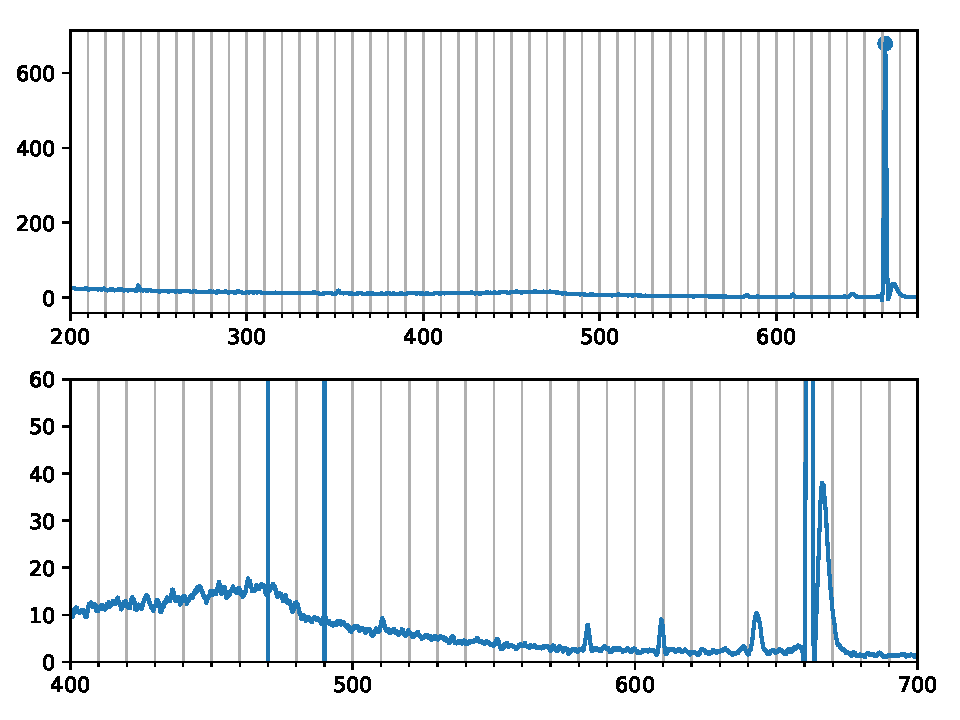
\includegraphics[scale=0.8]{figs/Cs137.pdf}
  \caption{Graf závislosti napětí odezvy vzorku na napětím budícím magnetické pole}
\end{figure}
\begin{figure}[h]
  \hspace*{-1em}
  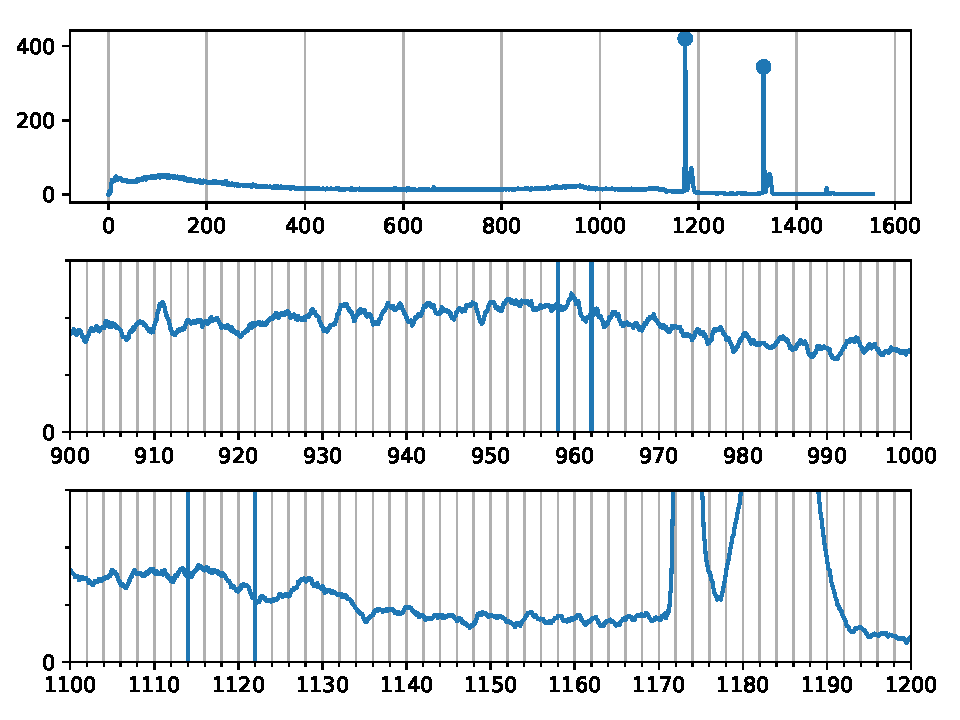
\includegraphics[scale=0.8]{figs/Co60.pdf}
  \caption{Graf závislosti napětí odezvy vzorku na napětím budícím magnetické pole}
\end{figure}
\begin{figure}[h]
  \hspace*{-1em}
  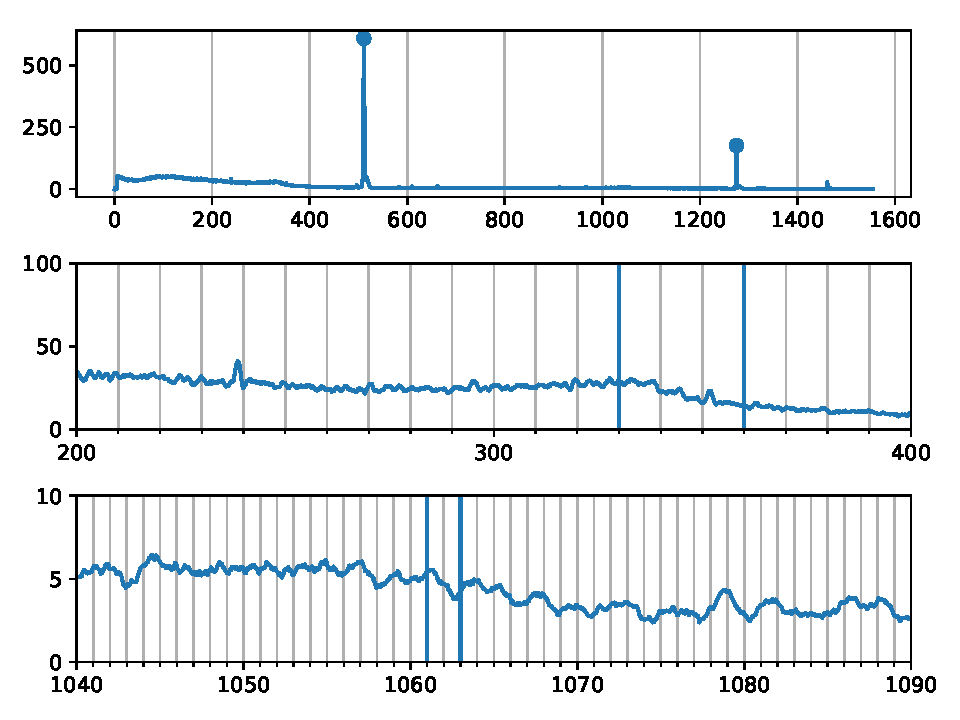
\includegraphics[scale=0.8]{figs/Na22.pdf}
  \caption{Graf závislosti napětí odezvy vzorku na napětím budícím magnetické pole}
\end{figure}
\begin{figure}[h]
  \hspace*{-1em}
  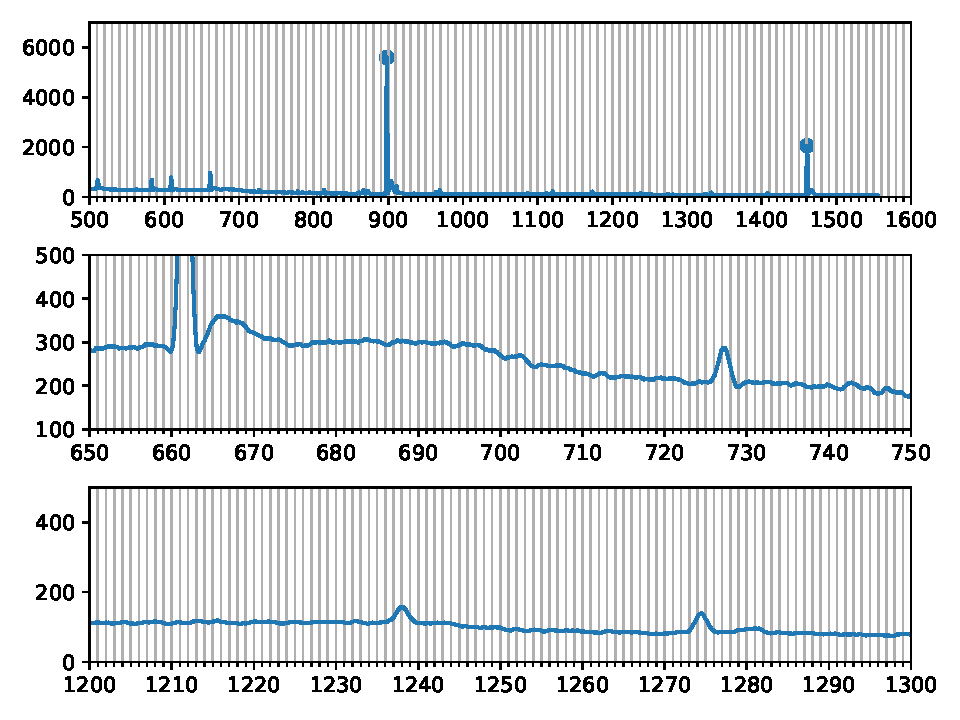
\includegraphics[scale=0.8]{figs/Y88.pdf}
  \caption{Graf závislosti napětí odezvy vzorku na napětím budícím magnetické pole}
\end{figure}
\end{document}
